\documentclass[tikz]{standalone}
\usepackage{amsmath,amssymb}

\newcommand{\twovec}[2]{\ensuremath{\begin{pmatrix}{#1}\\{#2}\end{pmatrix}}}
\newcommand{\V}[1]{\vec{\mathbf{#1}}}
\usetikzlibrary{patterns}
\tikzset{mydraw/.style={black,->}}
\tikzset{mynode/.style={scale=0.7}}

\begin{document}
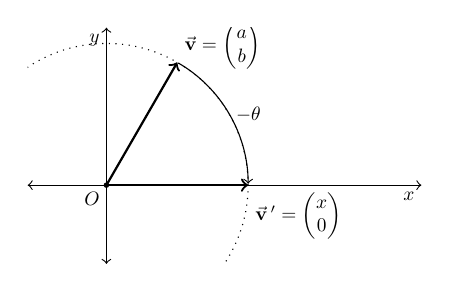
\begin{tikzpicture}
	\clip (-1,-1) rectangle (4,2);

	\draw[mydraw] (0,0) -- (-1,0);
	\draw[mydraw] (0,0) -- (0,-1);
	\draw[mydraw] (0,0) -- (4,0) node[mynode,below left] {\(x\)};
	\draw[mydraw] (0,0) -- (0,2) node[mynode,below left] {\(y\)}; % axis lines

	% Rotation hints
	\draw[dotted] (0,0) circle (1.8);
	\draw[mydraw,<-,shorten >=.5pt,shorten <=.5pt] (1.8,0) arc (0:60:1.8) node[mynode,midway,right] {\(-\theta\)};

	% Rotate and reflect
	\draw[rotate=60,thick,->] (0,0) -- (1.8,0) node[mynode,anchor=200] {\(\V{v} = \twovec{a}{b}\)};
	% Original basis
	\draw[thick,->] (0,0) -- (1.8,0) node[mynode,below right] {\(\V{v}\,' = \twovec{x}{0}\)};

	\fill[black] (0,0) circle (1pt) node[mynode,below left] {\(O\)};
\end{tikzpicture}
\end{document}
